\documentclass[a4paper]{article}
\usepackage[french]{babel}
\usepackage[utf8]{inputenc}
\usepackage[T1]{fontenc}
\usepackage{csquotes}   % pour éviter un warning
\usepackage{graphicx}   % pour les images
\usepackage{hyperref}   % pour les références
% \usepackage{amssymb}    % pour les symboles de maths comme \mathbb{R}
% \usepackage{mathtools}  % pour rajouter \text dans un environment math
% \usepackage{subcaption} % pour les subfigures
\usepackage{float}      % pour les figures

\usepackage[style=ieee,backend=biber]{biblatex}
\addbibresource{ref.bib}

\hypersetup{
    colorlinks=true,
    linkcolor=blue,   % Couleur des liens internes (table des matières, références)
    citecolor=green,  % Couleur des liens vers les références bibliographiques
    filecolor=magenta,% Couleur des liens vers les fichiers
    urlcolor=blue     % Couleur des liens vers les URL
}

\title{Rapport SAM \\ Modèle multi-modaux}
\author{Cléa Han, Yanis Labeyrie et Adrien Zabban}
\date{janvier 2024}

\begin{document}

\maketitle
\bigskip
\tableofcontents
\newpage

\section{Introduction}

Notre projet traite des approches multimodales pour la prédiction de changement de prise de parole dans des conversations naturelles. 
% Nous nous appuyons sur le corpus de données multimodales appelé Paco-Cheese~\cite{paperswithcode-paco}.
Les objectifs de ce projet nous permettent d'introduire différentes notions de modalité textuelle, visuelle et auditive, ainsi que de
comparer et d'explorer différents modèles de traitement multimodaux, et leur fusion entre eux.

\section{Données}
Les données proviennent d'un ensemble de données multimodales, en français, composé de 26 dyades de 15 à 20 minutes, 
corpus de données multimodales Paco-Cheese~\cite{paperswithcode-paco}.
Chaque dyade est composée de deux personnes qui discutent d'un sujet donné. Les données sont composées de trois modalités : la vidéo,
l'audio et le texte.

Le but du projet est, étant donné un bout de texte, audio et/ou vidéo, d'être capable de détecter le changement de parole.
On Peut alors voir ce problème comme un problème de classification de données à deux classes.

Nous avons coupé les données sur les IPUs (Inter-Pausal Units, voir l'article~\cite{turn-taking} pour plus d'information),
qui représentent des segments de parole séparés par des pauses
de plus de 200ms. À partir de chaque IPUs, nous allons récupérer les fins du flux vidéo, audio et de transcription du discours.
On a choisi de prendre les 20 derniers mots, les 2 dernières secondes de l'audio et les 10 dernières images du flux vidéos
(appartenant aux deux personnes pour l'audio et la vidéo).

Les données du flux vidéo ont été pré-process par un modèle permettant d'extraire les coordonnées de 709 points d'intérêts du 
visage, appelé landmarks. On a alors pour chaque image du flux vidéo, une liste de coordonnées représentent les landmarks. Cependant, 
du fait au grand nombre des données, leur analyse a été assez compliquée
\footnote{En effet, il y a 15 csv contenant chacun 30000 lignes et 700 colonnes. Ce qui fait que dans le dataloader, 
la récupération d'un item (récupération des 2 fois 10 images) nécessité d'ouvrir, parcourir le csv pour récupérer les bonnes lignes et
le refermer à la fin de l'itération (du au fait qu'on prend chaque item de manières aléatoire). On a quand même pu accélérer le processus
en utilisant la fonction \textit{skiprows} de \textit{pandas} qui permet de récupérer des lignes spécifiques dans un gros csv sans lire 
toutes les lignes mais cela n'a pas été suffisant.}

Chaque IPU est alors labellisé par un 0 ou un 1, selon s'il y a un changement de parole après ce moment. Il est important de noter que, 
comme on peut le voir dans la Table~\ref{tab: label distribution}, le dataset est fortement déséquilibré.

\begin{table}[H]
    \centering
    \begin{tabular}{|c|c|c|c|}
        \hline
        dataset & nombre d'IPUs & pourcentage de $0$ & pourcentage de $1$ \\
        \hline
        \textit{entraînement} & 8861 & 80.51 & 19.49\\
        \hline
        \textit{validation} & 3340 & 80.60 & 19.40\\
        \hline
        \textit{test} & 2974 & 82.85 & 17.15\\
        \hline
        \textit{tout} & 15175 & 80.99 & 19.01 \\
        \hline
    \end{tabular}
    \caption{Nombre d'IPU et distribution des labels sur les différents dataset.}
    \label{tab: label distribution}
\end{table}

\section{Traitement unimodale}
\subsection{Traitement du texte avec CamemBERT}

Pour parvenir à détecter le changement de tour de parole dans les données textuelles, nous avons choisi d'utiliser un modèle
considéré comme l'état de l'art pour la tâche de classification de texte : le modèle BERT (Bidirectional Encoder
Representations from Transformers~\cite{Bert}). Ce modèle utilise notament les Transformers~\cite{transformers} 
(voir son architecture Figure~\ref{fig: Transformers}).

Par ailleurs, BERT étant un modèle comprenant un nombre important de paramètres (environ 100 millions) il est inenvisageable avec
nos moyens de l'entraîner "à partir de 0". Nous avons donc opté pour l'utilisation d'un modèle pré-entrainé sur la langue Française
appelé CamemBERT et nous avons gelé les poids de CamemBERT.

\begin{figure}[H]
    \centering
    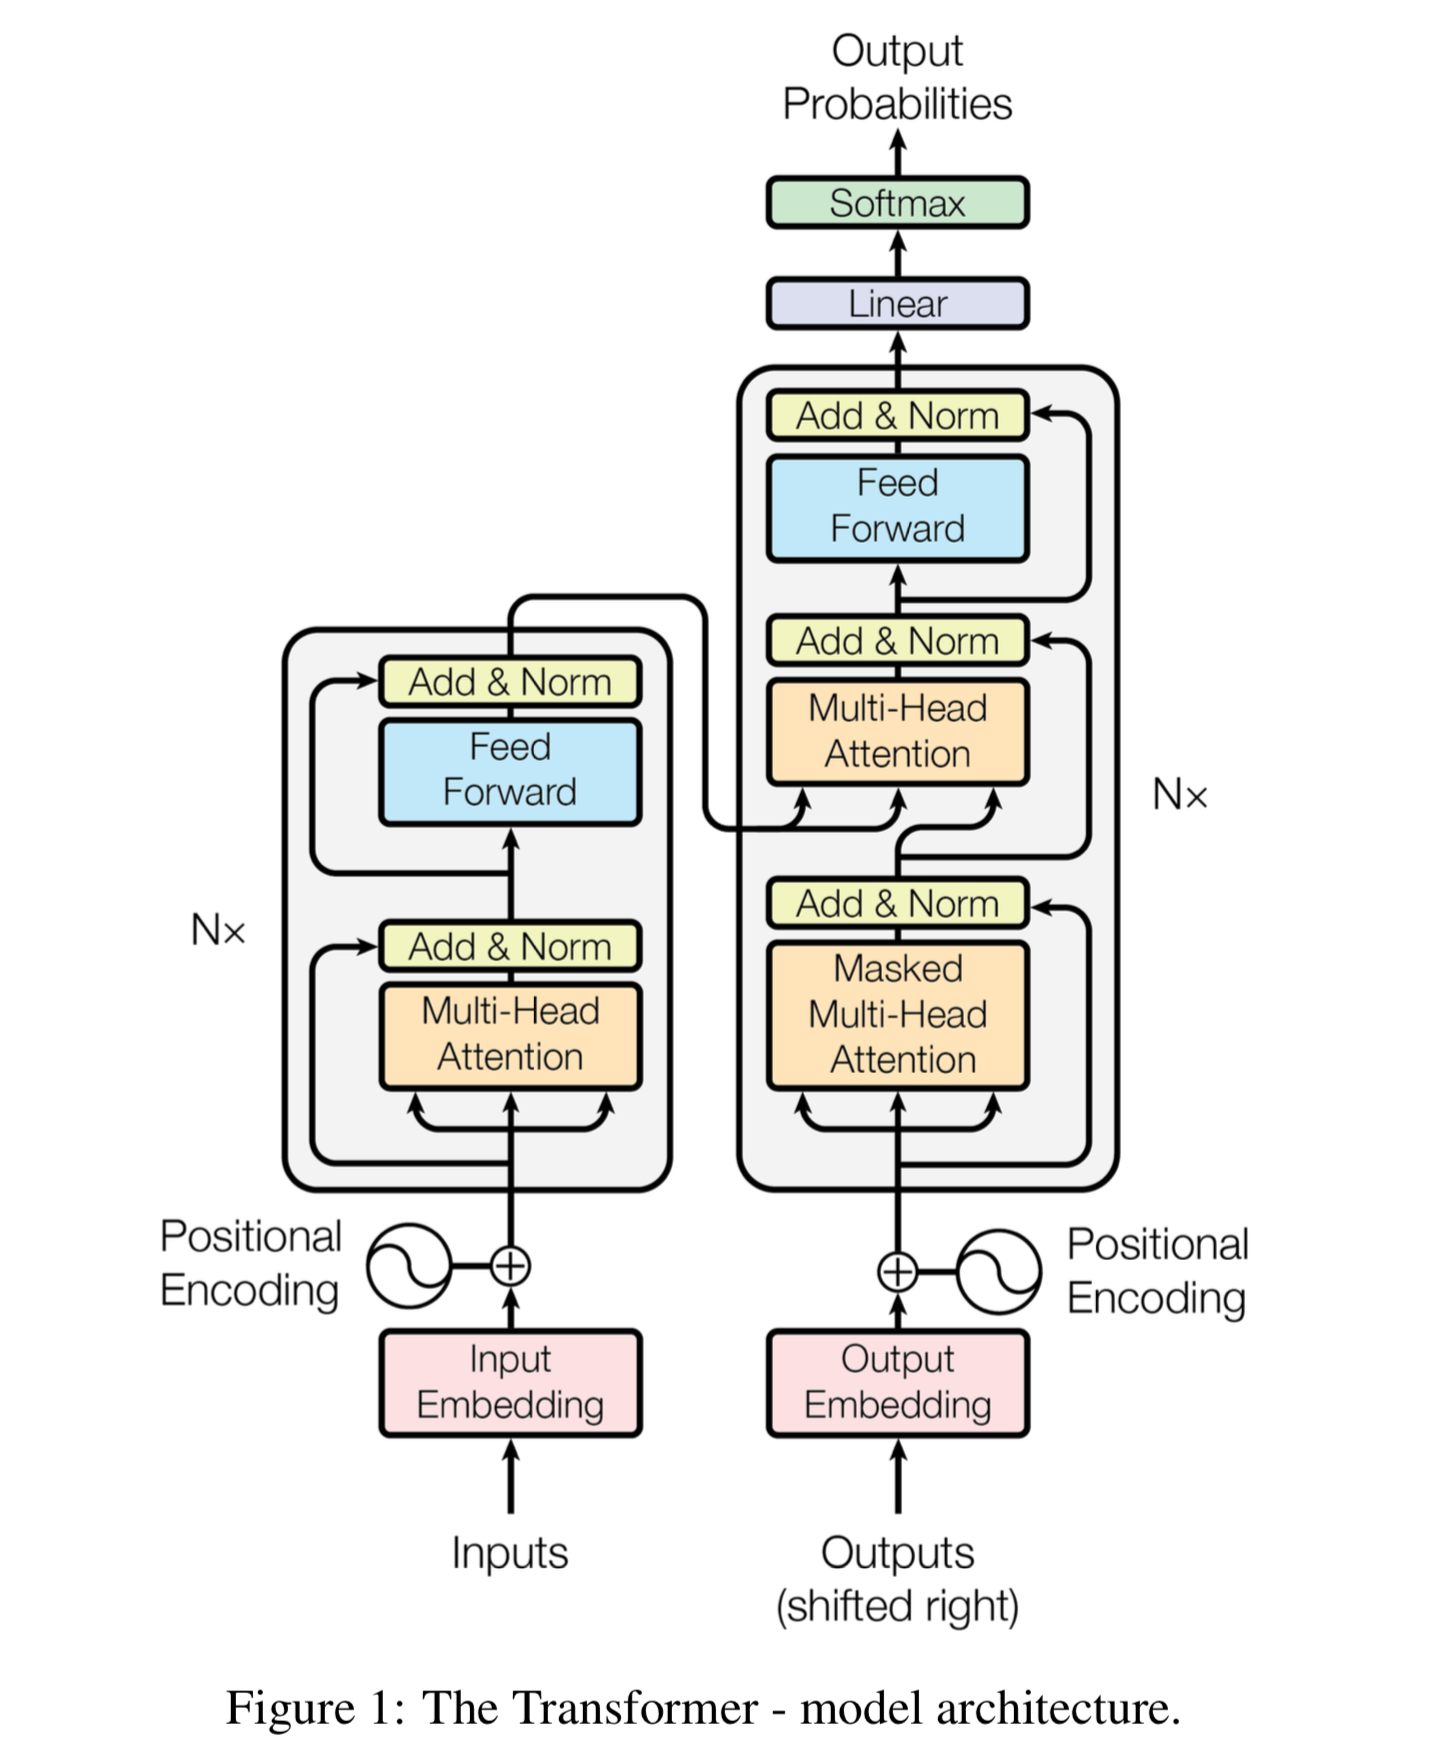
\includegraphics[width=0.6\textwidth]{image_model/model_transformers.png}
    \caption{Architecture de Transformers}
    \label{fig: Transformers} 
\end{figure}



On prend alors les données de textes qui sont une liste d'entiers, correspondant 
à l'indice de chaque mot du tokenizer de CamemBERT. Ces données passent alors dans CamemBERT, elles ressortent avec une dimension de
64. Elles passent alors dans une activation ReLU puis une couche dense de taille 64, puis une couche de dropout (avec un taux
d'oubli de $10\%$), pour enfin passer dans un dernier ReLU et une dernière couche dense à 2 dimensions. 
La Figure~\ref{fig: model_text} résume l'architecture de ce modèle, qu'on appelera \textit{TEXT}.

\begin{figure}[H]
    \centering
    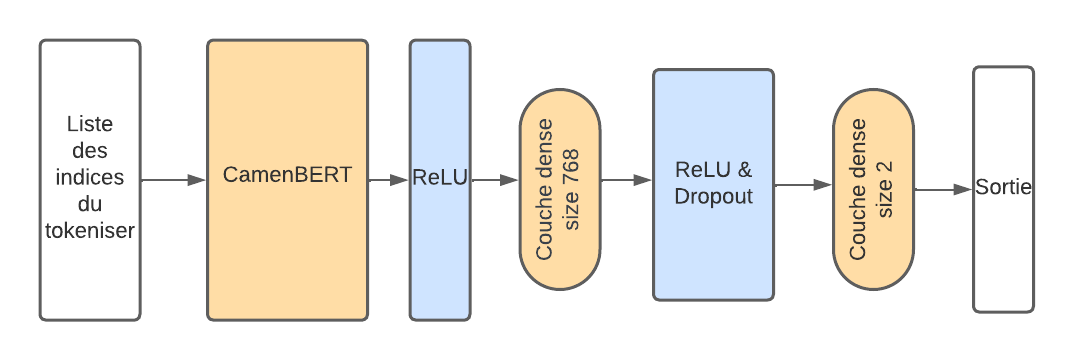
\includegraphics[width=0.7\textwidth]{image_model/model_text.png}
    \caption{Architecure du modèle \textit{TEXT}.}
    \label{fig: model_text}
\end{figure}

\subsection{Traitement de l'audio}

Afin de détecter les changements de parole dans des données audio, nous avons choisi d'exploiter une approche similaire en utilisant
un modèle avancé dans le domaine de la représentation audio : le modèle Wave2Vec~\cite{wav2vec}. Wave2Vec, basé sur les Transformers, s'est établi
comme une référence pour la tâche de traitement du signal audio, en particulier pour la détection des variations dans la parole.
Grâce à sa capacité à encoder de manière bidirectionnelle les représentations des signaux sonores, Wave2Vec excelle dans la
compréhension des nuances acoustiques et des transitions subtiles entre les locuteurs. 

On possède deux données en entrée qui sont les enregistrements audio des deux interlocuteurs. On fait alors passer leurs audio dans
Wave2Vec puis l'on concatène la sortie. On fait alors passer la concaténation dans une couche dense pour n'avoir qu'une sortie de
taille 2.
Eventuellement, ce modèle initial pouvait être amélioré en terme d'architecture, nous avons donc à l'issue de la concaténation,
ajouter une couche dense, puis une couche de ReLU et de dropout, et enfin finir sur une couche dense de sortie à 2 neurones. 
La Figure~\ref{fig: model_audio} résume l'architecture de ce modèle, qu'on appelera \textit{AUDIO}.

\begin{figure}[H]
    \centering
    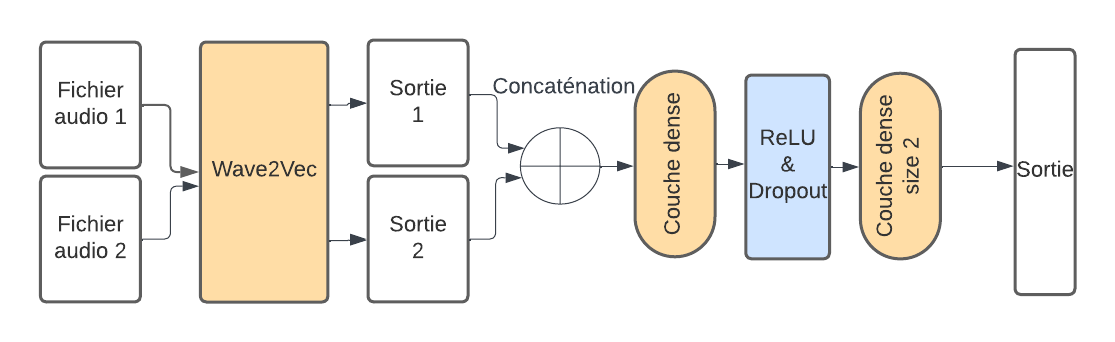
\includegraphics[width=0.7\textwidth]{image_model/model_audio.png}
    \caption{Architecure du modèle \textit{AUDIO}.}
    \label{fig: model_audio}
\end{figure}

\subsection{Traitement de la vidéo}

Pour traiter les données issues de la vidéo qui sont sous la forme des landmarks du visage des deux personnes en conversation,
nous avons choisi d'utiliser un réseau de neurones adapté à cette tâche d'analyse de séries temporelles : le réseau LSTM (Long-Short
Term Memory). En effet, ce modèle est pertinent pour la détection du changement de locuteur, car il est capable de conserver des
informations sur de longues séquences temporelles, ce qui est essentiel pour analyser les variations subtiles dans les mouvements
des landmarks faciaux. 

Comme pour l'audio, la vidéo contient un ensemble de deux fois 10 images pour chaque interlocuteur. On les fait alors passer
dans deux couches LSTM et on concatène les sorties pour ensuite les faire passer dans une couche ReLU et une couche dense de taille 2.
La Figure~\ref{fig: model_video} résume l'architecture de ce modèle, qu'on appelera \textit{VIDEO}.

\begin{figure}[H]
    \centering
    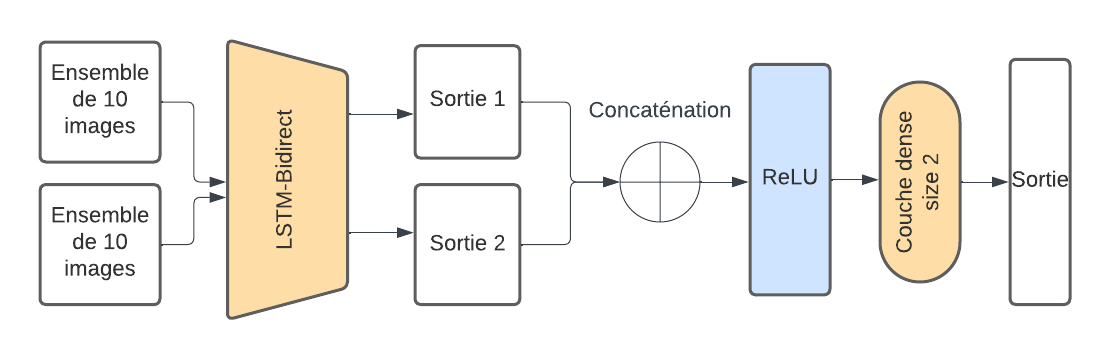
\includegraphics[width=0.7\textwidth]{image_model/model_video.png}
    \caption{Architecure du modèle \textit{VIDEO}.}
    \label{fig: model_video}
\end{figure}

\section{Traitement multimodal}
Notre approche vise à maximiser l'utilisation des dépendances et complémentarités entre différents types de données (vidéo, texte,
audio). Pour effectuer des prédictions en utilisant ces diverses modalités, nous avons opté pour l'utilisation de chaque réseau de
neurones présentés précédemment afin d'extraire des représentations compressées (ou features) des différents types de données. 

Les modèles individuels sont initialement pré-entraînés, puis fusionnés en une seule architecture multimodale qui subit ensuite un
nouvel entraînement. Le pré-entraînement des modèles individuels présente l'avantage de réduire le temps de convergence de
l'entraînement de cette architecture multimodale comprenant un nombre important de paramètres.

Au cours de ce processus, pour des raisons de contraintes de ressources, on gèle les poids des modèles unimodaux.

\subsection{Le LATE FUSION}
Ce premier modèle multimodal fait passer chaque donnée dans son modèle pré-entraîné associé et fait une moyenne des sorties. Le but
est alors de faire une moyenne des probabilités selon chaque canal. Nous appellerons ce modèle \textit{LATE FUSION}, du fait que la 
fusion se fasse à la fin. Comme ce modèle utilise seulement les modèles unimodaux pré-entrainés, il n'y a pas besoin de faire 
d'apprentissage sur ce modèle.
La Figure~\ref{fig: LATE FUSION} résume l'architecture de ce modèle.

\begin{figure}[H]
    \centering
    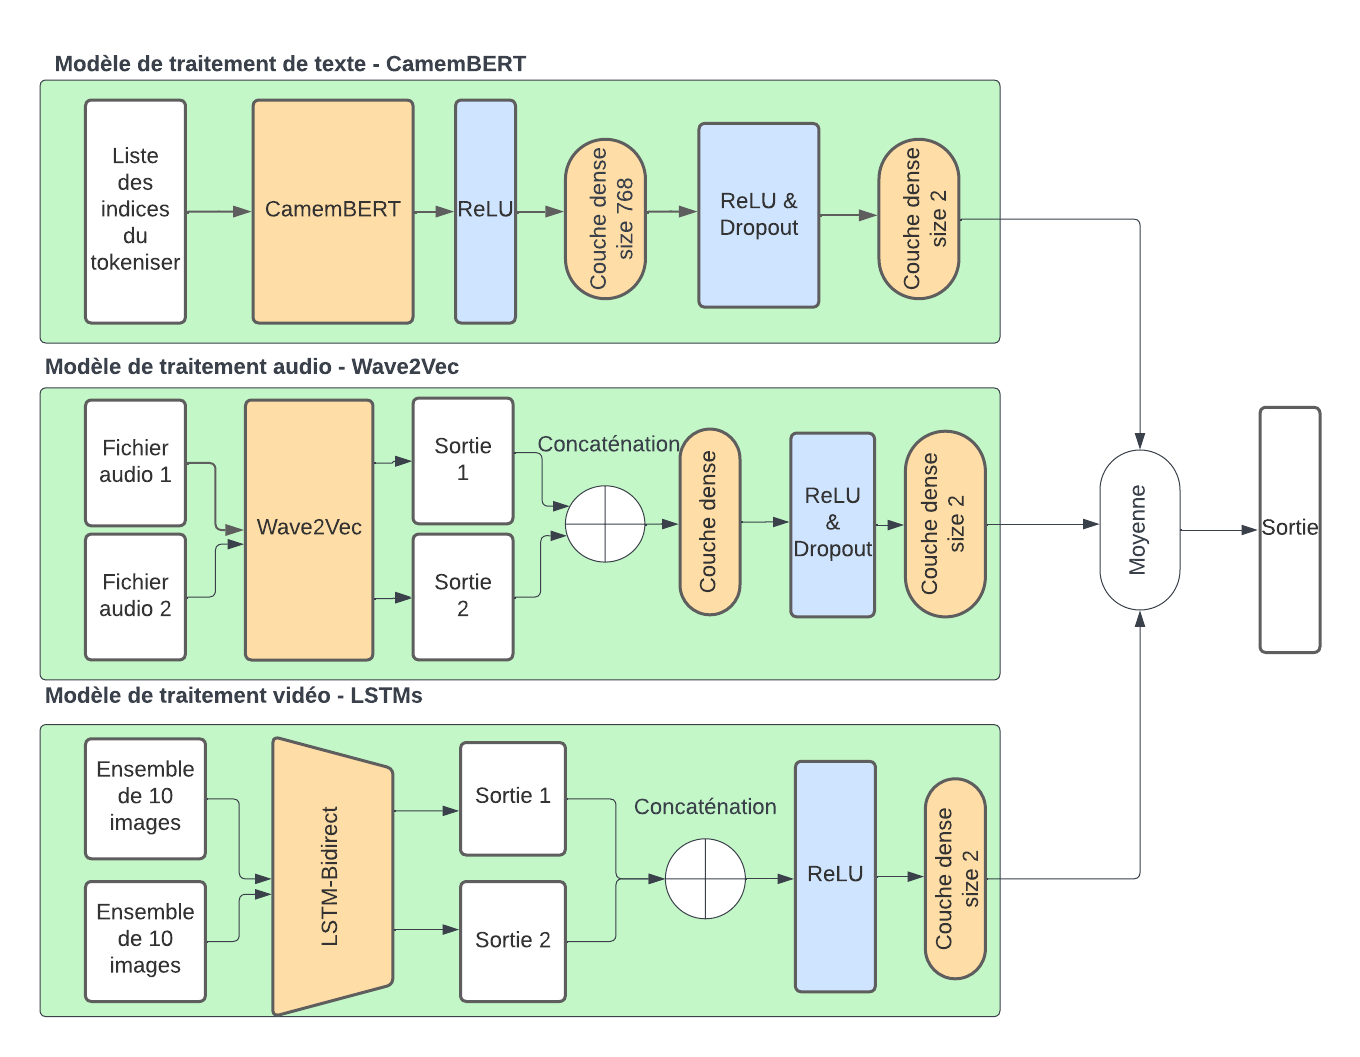
\includegraphics[width=0.6\textwidth]{image_model/late_fusion.png}
    \caption{Architecture du modèle \textit{LATE FUSION}}
    \label{fig: LATE FUSION}
\end{figure}

\subsection{L'EARLY FUSION}
Ce deuxième modèle plus évolué consiste à faire passer chaque donnée dans son modèle pré-entraîné associé et de récupérer
l'information avant qu'elle ne passe dans la dernière couche dense (celle de taille deux). On concatène alors toute l'information 
et on la fait passer dans une grande couche dense de taille 2.
La Figure~\ref{fig: EARLY FUSION} résume l'architecture de ce modèle, qu'on appellera \textit{EARLY FUSION}, du fait que la fusion
se passe avant les couches de neurones.

\begin{figure}[H]
    \centering
    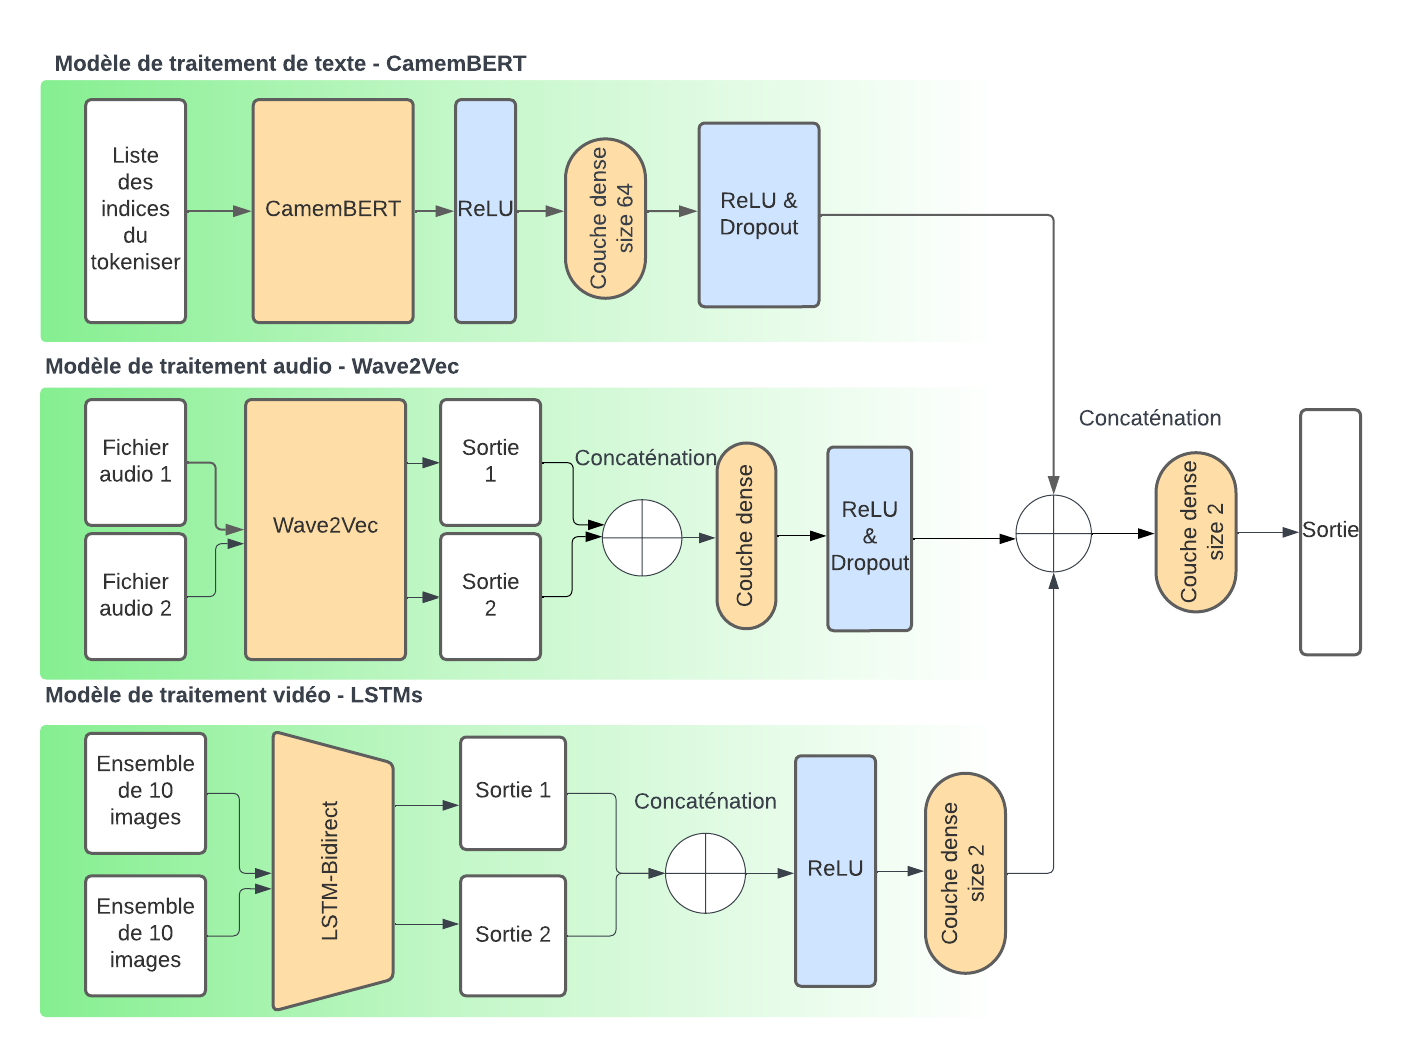
\includegraphics[width=0.6\textwidth]{image_model/early_fusion.png}
    \caption{Architecture du modèle \textit{EARLY FUSION}.}
    \label{fig: EARLY FUSION}
\end{figure}

\section{Entraînements}
Nous avons entraîné les modèles unimodaux et le \textit{EARLY FUSION}, sur 2 epochs, car ils utilisent tous (sauf \textit{VIDEO}), 
un modèle pré-entraîné, comment BERT ou Wave2Vec. Nous avons ensuite gardé les poids de 
l'epoch qui avait la plus basse loss de validation.

Cependant, l'entraînement du modèle \textit{VIDEO}, dû a la grandeur des données et 
leurs temps de chargement dans la RAM, nous avons décidé de faire qu'une seule epoch
\footnote{Une epoch durait plus de 2h30 sur google colab avec un GPU Nvidia T4.}, et de ne pas l'intégrer dans les modèles multimodaux.

\subsection{Loss et poids}
Nous avons utilisé la fonction de coût \textit{crossentropy} pour l'entrainement de modèles. 
Cependant, du fait, du fait du grand déséquilibré des classes (voir Table~\ref{tab: label distribution}), nous avons ajouté des poids 
sur les classes dans la fonction crossentropy. En effet, sans ces poids, les modèles avaient tendance à prédire toujours des $0$, ce 
qui leurs permetait d'optenir $80\%$ d'accuracy sans dificultés. Nous avons alors cherché des poids à mettre dans la loss de telle sorte 
que les modèles ne prédisaient pas systématiquement qu'un seul label
\footnote{Si on met un poids trop grand pour le label 1, même s'il y a que $20\%$ de $1$, les modèles vont prédire que des $1$.}.
Nous avons alors trouvé et appliqué les poids $w_0 = 1$ et $w_1=3.9$. La loss se calcule alors avec l'équation~\ref{eq: loss}
(avec des notations standards)~:

\begin{equation}
    L(x, y) = \frac{-1}{N} \sum_{n=0}^{N} w_0 (1-y_n) \log(1-x_n) + w_1 y_n \log(x_n)
    \label{eq: loss}
\end{equation}

\subsection{Métriques}
Pour comparer les résultats obtenus, nous avons utilisé la loss, mais aussi d'autres métriques,
comme l'accuracy, la précision, le rappel et le $f_1$-score.

Du fait des déséquilibres de classes, l'accuracy n'est pas les métriques la plus cruciale. On a donc opté pour 
calculer aussi la précision, le rappel et le $f_1$-score. Pour ces métriques, on a choisi de les calculer 
sur chacune des classes et d'en faire la moyenne. Ainsi un rappel de $0.3$ signifiera que la moyenne du rappel sur
la classe $0$ et la classe $1$ fasse $0.3$. Nous avons choisi de faire cela, car si l'on regardait seulement 
le rappel sur la classe $1$, le TRUE POSITIF (TP) est très souvent égale à $0$ et donc le rappel est nul. De même 
pour la précision et de $f_1$-score, ce qui nous apportait moins d'information.

\section{Résultats}
Après avoir entraîné les modèles, nous avons testé leurs performances sur la base de données de test.
La Figure~\ref{tab: test} nous alors les résultats des modèles en fonctions des métriques.

\begin{table}[H]
    \centering
    \begin{tabular}{|c|c|c|c|c|c|}
        \hline
        Modèle & accuracy & precision & rappel & $f_1$ score\\
        \hline
        \textit{TEXT} & 82.8 & 41.3 & 50.0 & 45.3\\
        \hline
        \textit{AUDIO} & 47.1 & 48.5 & 47.4 & 41.5\\
        \hline
        \textit{VIDEO} & \textbf{82.9} & 41.4 & 50.0 & 45.2\\
        \hline
        \textit{LATE FUSION} & 78.5 & \textbf{50.6} & 50.1 & \textbf{48.8}\\
        \hline
        \textit{EARLY FUSION} & \textbf{82.9} & 43.6 & \textbf{50.2} & 45.7\\
        \hline
    \end{tabular}
    \caption{Résultats de test des modèles. Le \textit{LATE} et \textit{EARLY FUSION} n'utilisent pas le modèle \textit{VIDEO}.}
    \label{tab: test}
\end{table}

Les modèles unimodaux de texte et vidéo performent de manière très satisfaisantes selon leur accuracy, mais moins bien selon les autres métriques.
Le modèle unimodal audio est moins bon globalement par rapport aux autres modèles unimodaux selon l'accuracy. 
Cependant, il performe de manière satisfaisante uniformément sur les différentes métriques d'accuracy, de précision, de rappel et de $f_1$ score. 

Le modèle unimodal de vidéo performe le mieux parmi les modèles unimodaux, en accuracy. Tandis que, les modèles multimodaux sont satisfaisants, voire même légèrement meilleurs globalement que les modèles unimodaux selon les différentes métriques. 
Les modèles unimodaux ont une tendance à mieux performer pour l'une des métriques proposées, tandis que les modèles multimodaux ont des performances plus homogènes parmi les différentes métriques utilisées. 

Selon l'accuracy, le modèle vidéo et le modèle \textit{EARLY FUSION} performent le mieux, celui-ci a également le meilleur score de rappel. Le modèle \textit{LATE FUSION} performe le mieux selon la précision et le $f_1$ score.


\section{Conclusion}

Notre projet a exploré l'utilisation de modèles unimodaux et du multimodaux pour l'analyse dynamique de la conversation en français.
Nos modèles unimodaux ont été entraînés sur des données textuelles, audio et vidéo séparément. 
Leurs performances variaient selon le type de données, avec des résultats prometteurs, selon des modalités différentes, pour les données textuelles, audio et vidéo.

Nos modèles multimodaux ont été entraînés en combinant les données textuelles et audio. 
Les résultats de ces modèles étaient comparables à ceux des meilleurs modèles unimodaux, ce qui indique que les données textuelles et audio contiennent des informations complémentaires.
C'est pour cela que les résultats des modèles multimodaux ont des performances plutôt similaires au modèle unimodal vidéo. 

Ces résultats suggèrent que les modèles multimodaux, en particulier ceux qui combinent les données textuelles et audio, peuvent être des outils efficaces pour analyser la dynamique conversationnelle. 

Comme perspective, on pourrait explorer différentes manières d'intégrer les trois modalités de données (textes, audios et vidéos) dans un modèle multimodal, 
ainsi que l'utilisation d'autres types de données ou de modèles d'apprentissage automatique. 

\newpage
\printbibliography

\end{document}
